 \subsubsection{UC5 - Visualizzazione beni e servizi}
  \begin{figure}[h]
 	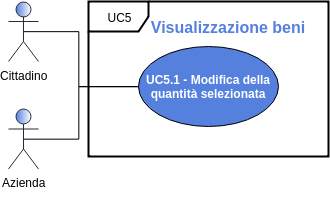
\includegraphics[width=6cm]{res/images/UC5-Generale.png}
 	\centering
 	\caption{UC6 - Gestione carrello}
 \end{figure}
 \begin{itemize}
 	\item \textbf{Attori Primari}: utente autenticato;
 	\item \textbf{Descrizione}: l'utente visualizza una lista dettagliata di informazioni relative ad un bene o servizio, esse comprendono la visualizzazione:
 	\begin{itemize}
 		\item del nome;
 		\item del prezzo lordo (in Cubit\glo);
 		\item della descrizione;
 		\item dell'immagine bene/servizio;
 		\item quantità di prodotto selezionata;
 	\end{itemize}
 	\item \textbf{Scenario principale}: l'utente si trova all'interno della pagina per la ricerca dei prodotti e sta visualizzando dei beni/servizi;
	\item \textbf{Inclusioni}:
	\begin{itemize}
		\item \textbf{UC16}: l'utente può filtrare i risultati visualizzati inserendo una parola chiave;
	\end{itemize}
 	\item \textbf{Precondizione}: l'utente, navigando nel sito, risulta all'interno di una pagina contenente almeno un bene o servizio;
 	\item \textbf{Postcondizione}: l'utente visualizza le informazioni relative al bene/servizio, con eventuali operazioni disponibili su di esso.
 \end{itemize}
 \subsubsection{UC5.1 - Modifica della quantità selezionata}
 \begin{itemize}
 	\item \textbf{Attori Primari}: cittadino, azienda\glo;
 	\item \textbf{Descrizione}: l'utente modifica la quantità del prodotto selezionato;
 	\item \textbf{Scenario principale}: l'utente modifica la quantità del prodotto selezionato utilizzando l'apposito campo;
 	\item \textbf{Precondizione}: l'utente sta visualizzando un prodotto ed intende modificarne la quantità selezionata;
 	\item \textbf{Postcondizione}: la quantità del prodotto è stata aggiornata al nuovo valore selezionato.
 \end{itemize}